\chapter{How we use Encryption}\label{encryption}

We may not realize this, but we use encryption every day.
The purpose of encryption is to keep us safe when we are browsing the internet or just storing our sensitive information on digital media.
In general encryption is used to secure our data, whether transmitted around the internet or stored on our hard drives, from being compromised.
Encryption protects us from many threats.

It protects us from identity theft.
Our personal information stored all over governmental authorities should be secured with it.
Encryption takes care for not revealing sensitive information about ourselves, to protect our financial details, passwords along with others, mainly when we bank online from being defraud.

It looks after our conversation privacy.
To be more specific, our cell phone conversations from eavesdroppers and our online chatting with acquaintances or colleagues.
It also allows attorneys to communicate privately with their clients and it aims to secure communication between investigation bureaus to exchange sensitive information about lawbreakers.

If we encrypt our laptop or desktop computer's hard drive encryption protects our data in case the computer or hard drive is stolen.

\section{Encryption and security}

Security is not binary; it is a sliding scale of risk management.
People are used to mark things, for example good and bad, expensive, and cheap.
But we know that people may differ on image/sense.
For example, there is no such thing as line or sign which tells us, this part of town is secure, and this is not.
The way we reason about security is that we study environment entering or observing it, and we begin to decide whether it is secure or not.
Especially at enterprise sector.
Encryption, on its own, might not be enough to make our data or infrastructure secure but is definitely a critical aspect of security.

Companies define their own security strategies which may include encryption or not at all.
Security strategies rely on company's needs or will to take risks in conclusion of getting high gain from them.

According to 2016 Global Encryption Trends Study, independently conducted by the Ponemon Institute, the enterprise-wide encryption in 5 years increased from 15 to 38 percent.
Also the ratio of companies with no encryption strategy at all decreased from 37 to 15 percent.
More than 50 percent companies are using extensively deployed encryption technologies to encrypt mostly databases, infrastructure and laptop hard drives \cite{Thales}.

Passwords are the most common authentication method used for accessing computer systems, files, data, and networks.
It is important to keep changing them in reasonable time and as a secret to others.
Still, no matter the company's security strategy, we keep seeing them on monitors or desktops written on sticky notes, and this is absolutely not secure.
In fact, users are the most vulnerable part of securing our systems.
To aid their memory, users often include part of a phone number, family name, Social Security number, or even birth date in their passwords \cite{pwdsec}.
They choose cryptographicaly weak passwords, dictionary words, which are easy to remember but also easy to guess or to break with brute-force attacks in short period of time.
According to Splash Data, a supplier of security applications, the most common user selected password in the year 2016 was "123456".
They claim that people continue to put themselves at risk for hacking and identity theft by using weak, easily guessable passwords.
To create strong password you can follow any trustworthy guide\footnote{https://www.wikihow.com/Create-a-Secure-Password} on the Internet. % https://www.centos.org/docs/4/html/rhel-sg-en-4/s1-wstation-pass.html\#S2-WSTATION-PASS-CREATE
More secure way to create passwords would be to generate cryptographically stronger cipher an use it as password.
The only disadvantage is that it is hard to remember \cite{splashdata}.

\section{Hard drive encryption}

It all starts, as mentioned, with desire to keep our data to ourselves and as a secret to others.
More often than not, these secrets are stored on our hard drives.

Hard drive encryption is a technology provided by software performing sophisticated mathematical functions or hardware that encrypts the data stored on a hard drive or a disk volume.
This technology is used to prevent unauthorized access by unauthorized persons or service to an encrypted data storage without possesion of the appropriate key or password.
Encrypting the hard drive means providing another layer of security against hackers and other online threats.

To protect secret data we usually encrypt this data by using an "encryption key" - see Figure \ref{fig:encdata} Hard drive encryption in a nutshell.
\begin{figure}[h]
    \centering
    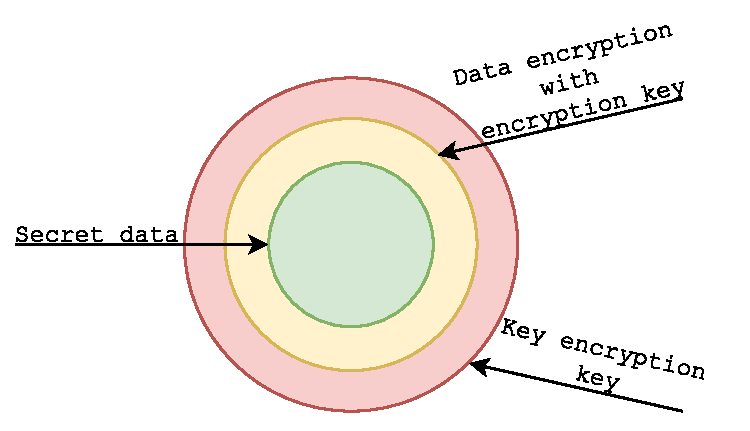
\includegraphics[scale=0.7]{figures/HowWeEncryptData.pdf}
    \caption{Hard drive encryption in a nutshell}
    \label{fig:encdata}
\end{figure}
Every encryption key should be unpredictable and unique set of bits able to "scramble" data in a way that it would be impossible to recover data whithout it.
To satisfy this need, encryption keys are generated by specialized algorithms such as AES (Advanced Encryption Standard\footnote{https://en.wikipedia.org/wiki/Symmetric-key\_algorithm\#Implementations}) for symmetric keys and RSA (Rivest–Shamir–Adleman\footnote{https://en.wikipedia.org/wiki/Public-key\_cryptography}) for asymmetric.
Changing encryption key implies the whole data decryption with old key and encryption with new encryption every time the old one is compromised or change is required.
Also this secret data might grow in size, and it is time and resource consuming to decrypt and encrypt the volume or even the whole hard drive.
Because of that the encryption key is then wrapped by the key encryption key.

Key encryption key is mostly generated using the user provided password.
This key encryption key is then used to encrypt encryption key which does the actual data encryption.
Again the most unsecure thing in this would be the user provided password which we can easily replace with using only cryptographically stronger key.
This principle has at least two advantages.
Changing the key encryption key does not affect encrypted data, and key can be changed whenever user desire to, and redistributed to all users or services who are supposed to access this data.

Hard drive could be encrypted as whole or per partition.
Full disk encryption is done in a way that all content on hard drive except MBR(Master Boot Record) is encrypted.
Encrypting MBR would make impossible to start boot sequence of the operating system.
Boot sequence would prompt user for key encryption key in order to load operating system from encrypted storage.

This could disrupt our daily basis and might be the reason why most of us do not use hard drive encryption, even when we know it will protect our data.
There is a way to automate hard drive unlocking on early boot with a help from key management system.
We can get the key encryption key from some remote system, the Escrow server mentioned in section \ref{escrow} Escrow server, or recover it with Tang described in chapter \ref{tang} Tang server.
Before that, let us have a look on most common hard drive encryption implementations.

\subsection{Bit Locker}
BitLocker is a closed source full disk data protection feature that integrates with the operating system Windows Vista and later.
It is designed to protect data by providing encryption for entire volumes and addresses the threats of data theft or exposure from lost, stolen, or inappropriately decommissioned computers.
By default it uses the AES encryption algorithm in cipher block chaining (CBC) or XTS mode with a 128-bit or 256-bit key.
CBC is not used over the whole disk; it is applied to each individual sector.

BitLocker supports TPM (Trusted Platform Module).
The TPM is a hardware component installed in many newer computers by the computer manufacturers.
It works with BitLocker to help protect user data and to ensure that a computer has not been tampered with while the system was offline\cite{bitlocker}.

\subsection{LibreCrypt}

LibreCrypt is a LUKS (Linux Unified Key Setup-on-disk-format) compatible open source “on-the-fly” transparent disk encryption software written mostly in Pascal programming language.
This project is based on original FreeOTFE project by Sarah Dean renamed in version 6.2 to LibreCrypt and supports both 32 and 64 bit Windows.
LibreCrypt is easy to use even for unexperienced user through its GUI (Graphical User Interface) with support of many languages.

LibreCrypt support many ciphers including AES (up to 256 bit), Twofish\footnote{https://en.wikipedia.org/wiki/Twofish} (up to 256 bit), Blowfish\footnote{https://en.wikipedia.org/wiki/Blowfish\_(cipher)} (up to 448 bit), Serpent\footnote{https://en.wikipedia.org/wiki/Serpent\_(cipher)} (up to 256 bit)\cite{librecrypt}.
It can create “virtual disks” on your computer and anything written to these disks is automatically encrypted before being stored on your computer’s hard drive\cite{FreeOTFE}.

Unfortunatelly this project seems to be abandoned by its developer on github.
The source code of LibreCrypt is available on GitHub you can visit the site or clone source code using~git:
\begin{lstlisting}[columns=fixed,basicstyle=\ttfamily\footnotesize,tabsize=4,backgroundcolor=\color{yellow!10}]
git clone https://github.com/t-d-k/LibreCrypt.git
\end{lstlisting}

\subsection{LUKS}

LUKS (Linux Unified Key Setup-on-disk-format) is a platform-independent disk encryption specification.
LUKS was created by Clemens Fruhwirth in 2004 and was originally intended for Linux distributions only.
It provides a standard on-disk-format for hard disk encryption, which facilitates compatibility among Linux distributions and provides secure management of multiple user passwords.

Referential implementation of LUKS is using a device-mapper crypt target (dm-crypt) subsystem for bulk data encryption.
This subsystem is not particularly bound to LUKS and can be used for plain format encryption.

It is important for us to know this specification a little more due to working with Linux distribution and the implemantation of the Tang server.

\section{Disk encryption with LUKS} \todo{merge and add motivation related to unlockers and tang}

With modern versions of cryptsetup (i.e., since ~2006), encrypted block devices can be created in two main formats, plain dm-crypt format or the extended LUKS format.

Plain format is just that: It has no metadata on disk.
When using any such encrypted device, all the necessary parameters must be passed to cryptsetup from the commandline (otherwise it uses the defaults, which will only succeed if the device was created using default settings).
It derives (generate) the master key from the passphrase provided and then uses that to decrypt or encrypt the sectors of the device, with a direct 1:1 mapping between encrypted and decrypted sectors.

In contrast to previous Linux disk encryption solutions, LUKS stores all necessary setup information in the partition header, enabling the user to more easily transport or migrate their data.
LUKS uses the dm-crypt subsystem.
Device-mapper is a part of the Linux kernel that provides a generic way to create virtual layers of block devices, most commonly LVM (Logical Volume Manager) logical volumes.
The device-mapper crypt target (dm-crypt) provides transparent encryption of block devices using the kernel crypto API (Application programming interface) supporting ciphers and digest algorithms via standard kernel modules.

In Fedora and Red Hat Enterprise Linux, userspace interaction with dm-crypt is managed by a tool called cryptsetup, which uses the device-mapper infrastructure to setup and operate on encrypted block devices.

The advantages of LUKS over plain dm-crypt are the higher usability: automatic configuration of non-default crypto parameters, the ability to add, change, and remove multiple passphrases.
Additionally, LUKS offers defenses against low-entropy passphrases like salting and iterated PBKDF2\footnote{https://en.wikipedia.org/wiki/PBKDF2} (Password-Based Key Derivation Function 2) passphrase hashing.
With LUKS, encryption keys are always generated by the kernel RNG (Random number generator); in contrast to plain dm-crypt where one can choose, e.g. a simple dictionary word and have an encryption key derived from that.
One disadvantage of using LUKS over plain is that it is readily obvious there is encrypted data on disk; the other is that damage to the header or key slots usually results in permanent data loss.
To mitigate this risk the Backup of the LUKS header would be best option \cite{fruhwirth2005luks}.

\subsection{Creating LUKS volume}\label{createLUKS}

Creating just a LUKS volume is quite easy all you need is tool called cryptsetup.
You can install it on Fedora system using command:
\begin{lstlisting}[columns=fixed,basicstyle=\ttfamily\footnotesize,tabsize=4,backgroundcolor=\color{yellow!10}]
# dnf install cryptsetup
\end{lstlisting}
Note, that this command has to be run by user with root privileges.
After installation succeeds all we need to do is to choose partition to encrypt.
For demonstration we will encrypt the {\it /dev/xvdc} patrtition using:
\begin{lstlisting}[columns=fixed,basicstyle=\ttfamily\footnotesize,tabsize=4,backgroundcolor=\color{yellow!10}]
# cryptsetup -y -v luksFormat /dev/xvdc
WARNING!
========
This will overwrite data on /dev/xvdc irrevocably.

Are you sure? (Type uppercase yes): YES
Enter LUKS passphrase:
Verify passphrase:
Command successful.
\end{lstlisting}
But having full disk encryption if the system is already installed might be quite tough.
Hard drive partition must contain the LUKS header just before the encrypted data.
Lets sum up the easier way first.

In case we have not installed our Linux operation system yet, we could simply select an option in time of installation.
Then the installation wizard will most likely asks for pass phrase - the key encryption key.
To demonstrate this, screen shots with Fedora 25 system installation can be found on appendix \ref{luksinstall} Pre-istallation enablement of hard drive encryption.

If we have already system installed with lots of data on partition, process will probably last longer and the procedure will be more complex.
There is no way you can encrypt whole system disk with LUKS without unmounting partition to encrypt.
For this purpose was developed {\it luksipc}, the LUKS In-Place Conversion Tool.
Steps to encrypt disk using {\it luksipc} are on appendix \ref{luksipc} LUKS In-Place Encryption.

\subsection{LUKS drive structure}

Hard drive with a LUKS partition has notable structure see Figure \ref{fig:luksvol} LUKS volume structure for demonstration.
The LUKS format uses a metadata header, also marked as {\it phdr}, and 8 key slot areas at the the beginning of the device.
After header there is section with bulk data, which are encrypted with the encryption key.
\begin{figure}[h]
    \centering
    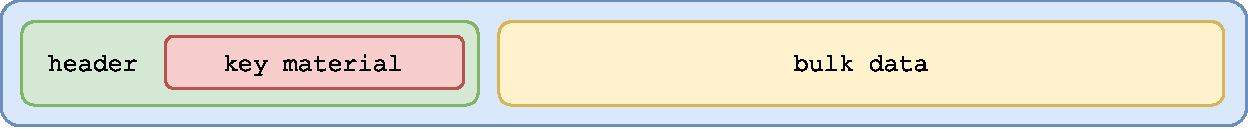
\includegraphics[scale=0.7]{figures/LUKSdrive.pdf}
    \caption{LUKS volume structure}
    \label{fig:luksvol}
\end{figure}
Header contains information about the used cipher, cipher mode, the key length, a uuid and a master key checksum.
The passphrases stored in the key slots, which structure is shown on Figure \ref{fig:luksslot} LUKS Key Slot, are used to decrypt a single key encryption key that is stored in the anti-forensic stripes.

\begin{figure}[h]
    \centering
    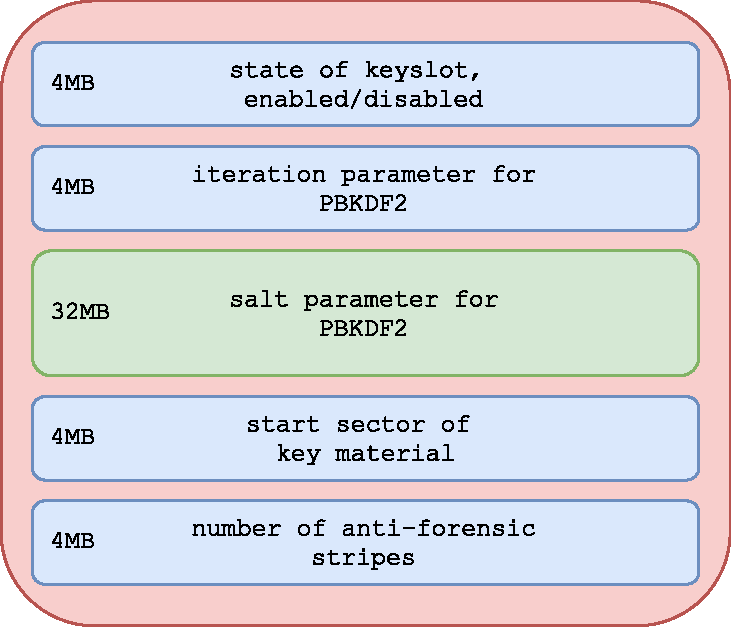
\includegraphics[scale=0.6]{figures/LUKSkeyslot.pdf}
    \caption{LUKS Key Slot}
    \label{fig:luksslot}
\end{figure}
Every key slot is associated with a key material section after the header.
When a key slot is active, the key slot stores an encrypted copy of the master key in its key material section.
This encrypted copy is locked by a user password or cipher.
Supplying this user password unlocks the decryption for the key material, which stores the master key.

\subsection{Managing LUKS volume}

This is demonstration how it could look like on real at this point our "host" Fedora 27 system.
For this demonstration we will use tools available for Fedora 27 such as:\\
\begin{itemize}
    \item parted-3.2-28.fc27.x86\_64
    \item cryptsetup-1.7.5-3.fc27.x86\_64
\end{itemize}
These tools are available through Fedora 27 upstream repositories and can be easily downloaded and installed via Fedora package management system the dnf.
To list hard drives for our system we will use the parted tool:
\begin{lstlisting}[columns=fixed,basicstyle=\ttfamily\footnotesize,tabsize=4,backgroundcolor=\color{yellow!10}]
# parted -l
Model: NVMe Device (nvme)
Disk /dev/nvme0n1: 256GB
Sector size (logical/physical): 512B/512B
Partition Table: msdos
Disk Flags:

Number  Start   End     Size    Type     File system  Flags
 1      1049kB  1075MB  1074MB  primary  ext4         boot
 2      1075MB  256GB   255GB   primary}
\end{lstlisting}
The exhibit shows that on our "host" system we have installed an NVMe (NVM Express) volume\footnote{https://en.wikipedia.org/wiki/NVM\_Express} using the msdos, therefore MBR partition table.
The NVMe is a specification for accessing SSDs attached through the PCI Express bus.
Our SSD drive has two partition as you can see the fist is boot partition and second should be our LUKS partition.
To find out if the second partition is LUKS volume we will use cryptsetup tool with option isLuks:
\begin{lstlisting}[columns=fixed,basicstyle=\ttfamily\footnotesize,tabsize=4,backgroundcolor=\color{yellow!10}]
# cryptsetup isLuks /dev/nvme0n1p1 -v
Device /dev/nvme0n1p1 is not a valid LUKS device.
Command failed with code 22: Invalid argument
\end{lstlisting}
This command has no /std/out nor /std/err output unless the -v option is used.
The actual result of the command is returned as exit code.
The output show reflects that our boot partition is not a valid LUKS volume as expected.
This is expected behavior, encrypting MBR partition would make impossible for system to boot.
\begin{lstlisting}[columns=fixed,basicstyle=\ttfamily\footnotesize,tabsize=4,backgroundcolor=\color{yellow!10}]
# cryptsetup isLuks /dev/nvme0n1p2 -v
Command successful.
\end{lstlisting}
At this point we have successfully identified the LUKS volume.
To dump the header information of this LUKS volume use cryptsetup option luksDump:
\begin{lstlisting}[columns=fixed,basicstyle=\ttfamily\footnotesize,tabsize=4,backgroundcolor=\color{yellow!10}]
# cryptsetup luksDump /dev/nvme0n1p2
LUKS header information for /dev/nvme0n1p2

Version:		1
Cipher name:	aes
Cipher mode:	xts-plain64
Hash spec:		sha256
Payload offset:	4096
MK bits:		512
MK digest:		85 b3 b9 71 b6 b7 51 18 60 39 78 db ac e8 82 97 0c 7b a2 3e
MK salt:		0d 22 53 83 56 0d a0 70 25 c2 bf fe 75 40 71 a9
				75 f1 ae a3 67 e5 b2 a5 14 85 39 1d c6 74 00 a8
MK iterations: 	52625
UUID:          	267c308e-5d64-4acf-abf2-f6e224e8febf

Key Slot 0: ENABLED
	Iterations:				415583
	Salt:		3e f9 7d 3b b6 08 60 9a eb dc 52 bb 8e 21 eb bf
				b9 4d 80 a4 70 2d 4e 97 8e 47 c1 a3 04 45 74 d4
	Key material offset:	8
	AF stripes:				4000
Key Slot 1: DISABLED
Key Slot 2: DISABLED
Key Slot 3: DISABLED
Key Slot 4: DISABLED
Key Slot 5: DISABLED
Key Slot 6: DISABLED
Key Slot 7: DISABLED
\end{lstlisting}
From the listing we can assume that /dev/nvme0n1p2 has one key encryption key in key slot 0 and has other 7 slots (1-7) disabled.
The advantage of LUKS is that if a team or group of up to eight people has to work with a common encrypted volume each team member may use his own password.
New user keys may be added to the encrypted volume and old user keys may be removed.
To add a new key we will use cryptsetup with option luksAddKey as shown:
\begin{lstlisting}[columns=fixed,basicstyle=\ttfamily\footnotesize,tabsize=4,backgroundcolor=\color{yellow!10}]
# cryptsetup luksAddKey  /dev/nvme0n1p2
Enter any existing passphrase:
Enter new passphrase for key slot:
Verify passphrase:
\end{lstlisting}
The cryptsetup will derive the key encryption key from this passphrase and bind it to first available key slot in LUKS header.
The dump of header will now contain information similar to the exhibit below:
\begin{lstlisting}[columns=fixed,basicstyle=\ttfamily\footnotesize,tabsize=4,backgroundcolor=\color{yellow!10}]
# cryptsetup luksDump /dev/nvme0n1p2
LUKS header information for /dev/nvme0n1p2

Version:		1
Cipher name:	aes
Cipher mode:	xts-plain64
Hash spec:		sha256
Payload offset:	4096
MK bits:		512
MK digest:		85 b3 b9 71 b6 b7 51 18 60 39 78 db ac e8 82 97 0c 7b a2 3e
MK salt:		0d 22 53 83 56 0d a0 70 25 c2 bf fe 75 40 71 a9
				75 f1 ae a3 67 e5 b2 a5 14 85 39 1d c6 74 00 a8
MK iterations: 	52625
UUID:			267c308e-5d64-4acf-abf2-f6e224e8febf

Key Slot 0: ENABLED
	Iterations:				415583
	Salt:		3e f9 7d 3b b6 08 60 9a eb dc 52 bb 8e 21 eb bf
				b9 4d 80 a4 70 2d 4e 97 8e 47 c1 a3 04 45 74 d4
	Key material offset:	8
	AF stripes:				4000
Key Slot 1: ENABLED
	Iterations:				1247257
	Salt:		44 48 92 df 29 8a df 81 f6 44 f8 66 c5 c2 32 49
				23 76 8a 37 48 85 33 2a 29 10 d8 cc 8f 45 0a 46
	Key material offset:	1520
	AF stripes:				4000
Key Slot 2: DISABLED
Key Slot 3: DISABLED
Key Slot 4: DISABLED
Key Slot 5: DISABLED
Key Slot 6: DISABLED
Key Slot 7: DISABLED
\end{lstlisting}
At this point LUKS volume is accessible via two different passphrases.
To remove any key from LUKS header we will use cryptsetup with option luksKillSlot as shown:
\begin{lstlisting}[columns=fixed,basicstyle=\ttfamily\footnotesize,tabsize=4,backgroundcolor=\color{yellow!10}]
# cryptsetup luksKillSlot /dev/nvme0n1p2 0
Enter any remaining passphrase:
\end{lstlisting}
To successfully remove key from key slot 0 we have to enter any remaining passphrase.
In our case we would enter the newly created passphrase which is bound to key slot 1.
This will result into having LUKS header in state like shown:
\begin{lstlisting}[columns=fixed,basicstyle=\ttfamily\footnotesize,tabsize=4,backgroundcolor=\color{yellow!10}]
# cryptsetup luksDump /dev/nvme0n1p2
LUKS header information for /dev/nvme0n1p2

Version:		1
Cipher name:	aes
Cipher mode:	xts-plain64
Hash spec:		sha256
Payload offset:	4096
MK bits:		512
MK digest:		85 b3 b9 71 b6 b7 51 18 60 39 78 db ac e8 82 97 0c 7b a2 3e
MK salt:		0d 22 53 83 56 0d a0 70 25 c2 bf fe 75 40 71 a9
				75 f1 ae a3 67 e5 b2 a5 14 85 39 1d c6 74 00 a8
MK iterations: 	52625
UUID:			267c308e-5d64-4acf-abf2-f6e224e8febf

Key Slot 0: DISABLED
Key Slot 1: ENABLED
	Iterations:				1247257
	Salt:		44 48 92 df 29 8a df 81 f6 44 f8 66 c5 c2 32 49
				23 76 8a 37 48 85 33 2a 29 10 d8 cc 8f 45 0a 46
	Key material offset:	1520
	AF stripes:				4000
Key Slot 2: DISABLED
Key Slot 3: DISABLED
Key Slot 4: DISABLED
Key Slot 5: DISABLED
Key Slot 6: DISABLED
Key Slot 7: DISABLED
\end{lstlisting}
Password rotation is very important.
To change LUKS key slot passphrase use the cryptsetup's option luksChangeKey:
\begin{lstlisting}[columns=fixed,basicstyle=\ttfamily\footnotesize,tabsize=4,backgroundcolor=\color{yellow!10}]
#cryptsetup luksChangeKey /dev/nvme0n1p2 -S 1
Enter passphrase to be changed:
Enter new passphrase:
Verify passphrase:
\end{lstlisting}
Note that passphrase to be changed and the slot number must be related to each other.
We could see change in LUKS header after command succeeded:
\begin{lstlisting}[columns=fixed,basicstyle=\ttfamily\footnotesize,tabsize=4,backgroundcolor=\color{yellow!10}]
# cryptsetup luksDump /dev/nvme0n1p2
LUKS header information for /dev/nvme0n1p2

Version:		1
Cipher name:	aes
Cipher mode:	xts-plain64
Hash spec:		sha256
Payload offset:	4096
MK bits:		512
MK digest:		85 b3 b9 71 b6 b7 51 18 60 39 78 db ac e8 82 97 0c 7b a2 3e
MK salt:		0d 22 53 83 56 0d a0 70 25 c2 bf fe 75 40 71 a9
				75 f1 ae a3 67 e5 b2 a5 14 85 39 1d c6 74 00 a8
MK iterations: 	52625
UUID:			267c308e-5d64-4acf-abf2-f6e224e8febf

Key Slot 0: DISABLED
Key Slot 1: ENABLED
	Iterations:				1630572
	Salt:		cf 54 a9 77 ed 8b c5 75 ca 65 60 6b 31 cb 29 0f
				4e 54 78 8c b1 9a db 3f 2f 6c aa 84 79 da 81 66
	Key material offset:	512
	AF stripes:				4000

Key Slot 2: DISABLED
Key Slot 3: DISABLED
Key Slot 4: DISABLED
Key Slot 5: DISABLED
Key Slot 6: DISABLED
Key Slot 7: DISABLED
\end{lstlisting}
For more usecases and examples how to use cryptsetup see the man page of the tool\footnote{https://linux.die.net/man/8/cryptsetup}.
Examples shown demonstrate basic key management for LUKS volumes and should be sufficient for basic understanding of cryptsetup/LUKS behavior and usability on the system with encrypted drive.
\todo{nafuknut little bit}

\subsection{LUKS security}

In August 2012 Ubuntu Privacy Remix Team did a deep analysis of LUKS/cryptsetup in Ubuntu enviroment.
Cryptsetup in version 1.4.1 used by Ubuntu 12.04 LTS has been chosen for they analysis.
They wrote the programs luksanalyzer and hashtest for the purpose of the analysis.

At the end they came into conlusion that cryptsetup with LUKS is a highly secure program for encrypting whole data media or partitions thereupon.
The encryption algorithms and other security mechanism it implements comply with the current state of the art in cryptography.
They found no back door or security-related mistake in the published source code.
If we use this program in a secure environment we may assume with high certainty that no one can get access to the data stored in your volumes as long as they are closed, the passwords are really good and the attacker doesn't apply highly advanced methods below the layer of the operation system, such as BIOS rootkits, hardware keyloggers or video surveillance.
A special strong point of Cryptsetup with LUKS is its high power of resistance against dictionary attacks.
This resisting power is adapted to the increased speed of hardware when new encrypted volumes are created on new up to date hardware\cite{team2012security}.
